\documentclass[journal=jpcafh,manuscript=article,layout=onecolumn, 12pt]{achemso}
\usepackage[version=3]{mhchem} % Formula subscripts using \ce{}
\usepackage[T1]{fontenc}       % Use modern font encodings
\usepackage{amsmath}
\usepackage[dvipsnames]{xcolor}
% NB added command for in line cite
\newcommand{\onlinecite}[1]{\hspace{-1 ex} \nocite{#1}\citenum{#1}} 
%
\author{Benjamin~A.~Laws}
\affiliation{School of Chemistry, University of New South Wales, Sydney NSW 2052, Australia}
\author{Olha Krechkivska}
\affiliation{School of Chemistry, University of New South Wales, Sydney NSW 2052, Australia}
\author{Callan M. Wilcox}
\affiliation{School of Chemistry, University of New South Wales, Sydney NSW 2052, Australia}
\author{Klaas Nauta}
\affiliation{School of Chemistry, University of New South Wales, Sydney NSW 2052, Australia}
\author{Scott H. Kable}
\affiliation{School of Chemistry, University of New South Wales, Sydney NSW 2052, Australia}
\author{Timothy~W.~Schmidt} 
\email{timothy.schmidt@unsw.edu.au}
\affiliation{School of Chemistry, University of New South Wales, Sydney NSW 2052, Australia}
\alsoaffiliation{ARC Centre of Excellence in Exciton Science, Australia}
\title{Intramolecular Hole$-$Transfer in Protonated Anthracene}
\abbreviations{PES,PAD,EA,eKE,FWHM,VMI}
\begin{document} 
\begin{abstract} 
doo doo doo
\end{abstract}
\section{Introduction}
Charge transfer between two different molecules in an excited electronic state is at the heart of photosynthesis. This process is also mimicked in artificial devices which generate solar energy. In both organic photovoltaics (OPV) and dye-sensitized solar cells, following photon absorption, the excited state migrates and undergoes a charge transfer event. A detailed understanding of charge separation in OPV is hampered, in part, by the impossibility of detailed quantum chemical calculations on such a large system. In OPV devices, the electrons and holes are then conducted to metallic electrodes through a series of inter and intramolecular electron and hole-transfer processes.

Gas-phase laser spectroscopy offers the possibility to interrogate a well-defined, cold, isolated chemical system which is tractable at quantitative levels of electronic structure theory. To study photo-induced hole-transfer, a charged species must be studied, which engenders further experimental difficulties. Cations can be introduced into the gas phase by electrospray ionization, but the resulting species are not cold. Jet-cooled molecules can be ionized in the expansion region, but unless the ionization is at threshold, requiring tunable vacuum ultraviolet radiation, excess energy can be deposited in the cation. Techniques capable of studying jet-cooled, isomer-selected, cold cations are thus desirable.

The C$_{60}^+$ cation was recently studied by the photodissociation of its adduct with helium atoms in a 22-pole cryogenic ion trap. This technique affords a spectrum with a very small shift from the true gas phase spectrum. For C$_{60}^+$ cation this was sufficiently small to confirm the present of C$_{60}^+$ in interstellar space~\cite{cam15}. Recently, we reported a triple-resonance technique whereby nascent cations were resonantly photodissociated following preparation by a resonant 2-colour 2-photon photon ionization process, at threshold. The result was an unambiguous spectrum of protonated naphthalene, isomer selected and vibrationally cold~\cite{kre13}. Here we extend this treatment to protonated anthracene, which demonstrates symmetry-breaking in the excited state along a Marcus-Hush-like charge transfer coordinate.

%Protonated polyaromatic cations PAH+ are also of considerable interest to astrochemistry, as their abundance in the interstellar medium (ISM) makes them promising candidates for diffuse interstellar band (DIB) carriers~\cite{mey21}. %While early photostability studies suggested that only relatively large (>50 C atoms) PAH molecules could survive in the ISM~\cite{joc94}, more recent studies have shown that structure also plays an important role. A Photoionization Mass Spectrometry experiment of a variety of PAHs showed that the Anthracene structure was relatively photostable, and is predicted to survive in regions of the ISM~\cite{joc99}. Despite this interest in



Protonated anthracene has been studied previously, as its relatively high photostability~\cite{joc99} and abundance in the interstellar medium (ISM) suggest it is a promising diffuse interstellar band (DIB) carrier candidate~\cite{mey21}. However, previous reports are neither at rigorously low vibrational temperature, nor isomer-selected. Alata \emph{et al.} measured the photo-fragmentation spectra of protonated anthracene, which was created (along with other PAHs) in an electrical discharge containing H$_2$~\cite{ala10}. Through comparison to RI-MP2 calculations, structure observed around 491~nm was assigned to the $\text{S}_0\rightarrow \text{S}_1$ transition of the 9H-An+ isomer. A subsequent absorption measurement of protonated anthracene held in a cryogenic matrix by Garkusha~\emph{et al.} exhibited several spectral bands across the 400-500nm region~\cite{gar11}. They instead assigned the structure around 491~nm to the $\text{S}_0\rightarrow \text{S}_2$ transition of the 1H-An+ isomer, based on TD DFT B3LYP calculations. A recent computational study has suggested the initial assignment to the 9H-An+ isomer was correct, however this discrepancy highlights the need for isomer selectivity~\cite{li21}. Electronic spectra of protonated anthracene have also been measured via helium-tagging action spectroscopy, however this technique is also limited by isomer non-selectivity and spectral resolution~\cite{mey21}.

In this study, we prepare 9-hydroanthracenium cations exclusively in their vibrational ground state by 2-color resonant ionization of the corresponding 9-dihydroanthracenyl radical. Subsequent resonant photodissociation of the cation reveals the isomer-selected $\text{S}_0\rightarrow\text{S}_1$ spectrum of 9-hydroanthracenium. We show that the $C_{2v}$ ground state undergoes symmetry breaking in the excited state along a $b_2$ (in-plane) mode, effectively localizing the positive charge on one end of the molecule. This coordinate thus represents the abscissa of a Marcus diagram, and the excitation spectrum is interpreted from this standpoint.

\section{Theoretical Considerations}
Anthracene protonated at the 9-position is considered $C_{2v}$ until proven otherwise. If the sp$^3$ carbon is considered as an insulator, the chromophore will consist of two aromatic rings linked by an sp$^2$-hybridized bridging carbon. The frontier orbitals of the aromatic rings can be taken in even and off combinations, resulting in sets of $b_1$ and $a_2$ symmetry. Only the $b_1$ set can interact with the bridge, which is also $b_1$. Of the highest occupied aromatic $b_1$ orbitals, one will have a node at the tertiary carbon atom adjacent to the bridge, and is not expected to be strongly perturbed. The other mixes with the bridging p-orbital and is lowered in energy. This results in two relatively unperturbed aromatic, symmetry-adapted orbitals of $a_2$ and $b_1$ symmetry. The lowest-energy unoccupied orbital is largely located on the bridge. The frontier orbitals are shown in Figure~\ref{Fig:1}.

\begin{figure} [h]
	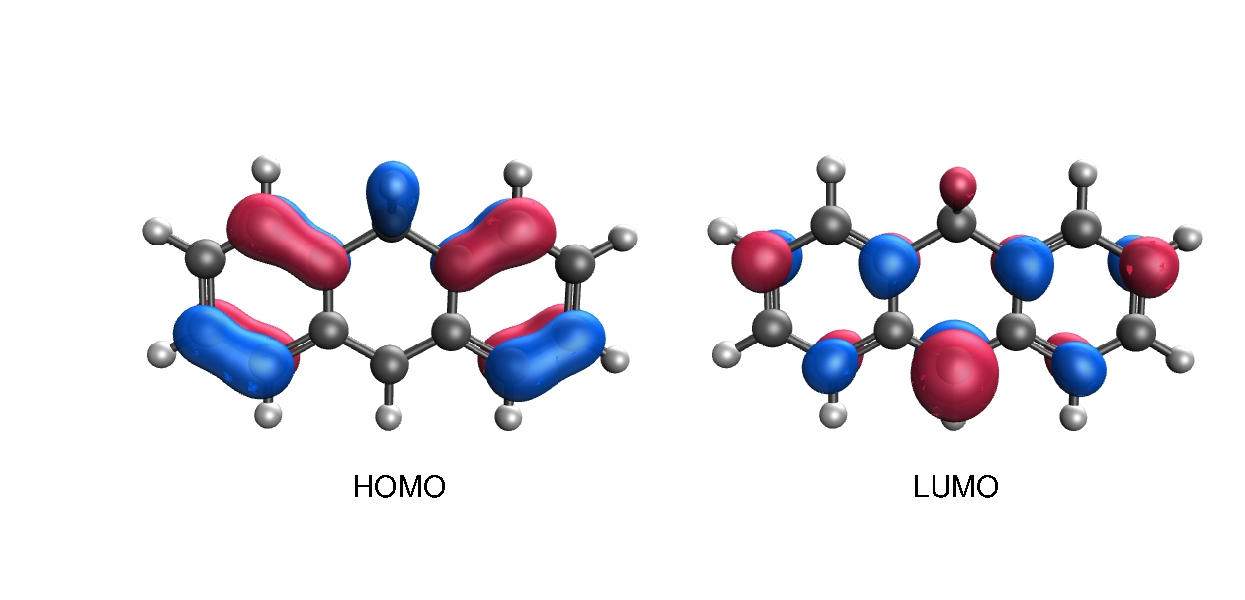
\includegraphics[width=0.2\textwidth]{figures/Figure1}
	\caption{goat}
	\label{Fig:1}
\end{figure}

The HOMO-LUMO transition of the cation is thus electron transfer from the aromatic rings to the bridge, corresponding to hole-transfer from the bridge onto the aromatic rings. This brings about two near-degenerate transitions to states of $A_1$ and $B_2$ symmetry. Distortion along a $b_2$ mode will reduce the point group to $C_s$ and render both these excited states $A'$. The interaction between these two states could potentially push the lower state to an energy below that of the $C_{2v}$ geometry.

This was confirmed by quantum chemical calculations presented in this work. The ground state geometry was calculated at both the M06-2X/cc-pvtz and CCSD/cc-pvdz levels of theory, with both calculations converging to a planar $C_{2v}$ geometry. All frequencies were found to be real, indicating a true minimum energy. Corresponding TDDFT and EOM-CCSD excited state calculations were also computed for the S$_1$ state, which converged to a planar $C_s$ geometry. This geometry arises from the charge transfer from the bridge onto one of the aromatic rings, causing an in-plane $b_2$ distortion. To interrogate this charge transfer process, a transition state search on the S$_1$ surface was also carried out at the M06-2X/cc-pvtz level using the Berny algorithm of Gaussain16. This found a $C_{2v}$ geometry with one imaginary frequency, 35~cm$^{-1}$ above the $C_s$ ground state.

The pathway from the $C_{2v}$ to $C_s$ geometry can be described by the intrinsic reaction coordinate (IRC). This was calculated in both the forward and reverse directions using Gaussian16 software and the HPC algorithm, calculating force constants at each step along the path. This produced a shallow double well potential, as shown in Figure~\ref{Fig:2}(a). The potential energy surface is shown across both the forward and reverse IRC directions, highlighting the $C_{2v}$ saddle point and the two $C_s$ global minima. The coordinate between the minima represents the charge hoping between the two aromatic rings. The higher excited $S_2$ and $S_3$ electronic state energies were also calculated along the IRC coordinate, as shown in Figure~\ref{Fig:2}(b). The surfaces resemble an avoided crossing, which suggests there may be a strong adiabatic interaction between the $S1~(^1A_1)$ and $S2~(^1B_2)$ states.  

\begin{figure} [h]
	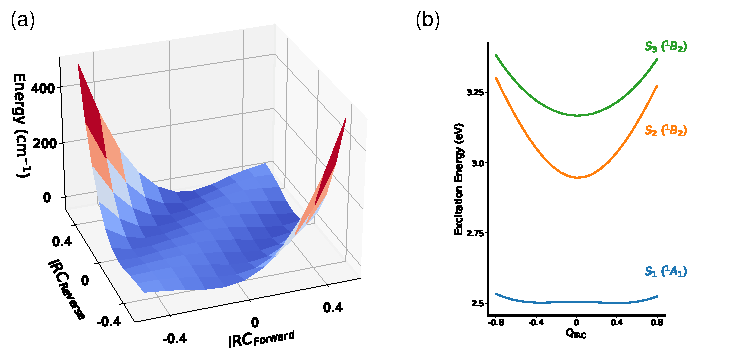
\includegraphics[width=0.8\textwidth]{figures/Figure2}
	\caption{cat}
	\label{Fig:2}
\end{figure}

To visualise the charge transfer, electrostatic potential surfaces were evaluated at both the $C_{2v}$ and $C_s$ geometries, as shown in Figure~\ref{Fig:3}. The surfaces show that the positive charge largely resides on the $sp2$ bridge at the ground state $C_{2v}$ geometry. During excitation to the $S1$ state, the hole hops onto one of the aromatic rings, where it remains localised at the excited $C_s$ geometry. This demonstrates that the shallow double well represents the abscissa of a Marcus charge transfer diagram, making protonated anthracene an excellent prototype for the study of intramolecular hole$-$transfer.

\begin{figure} [h]
	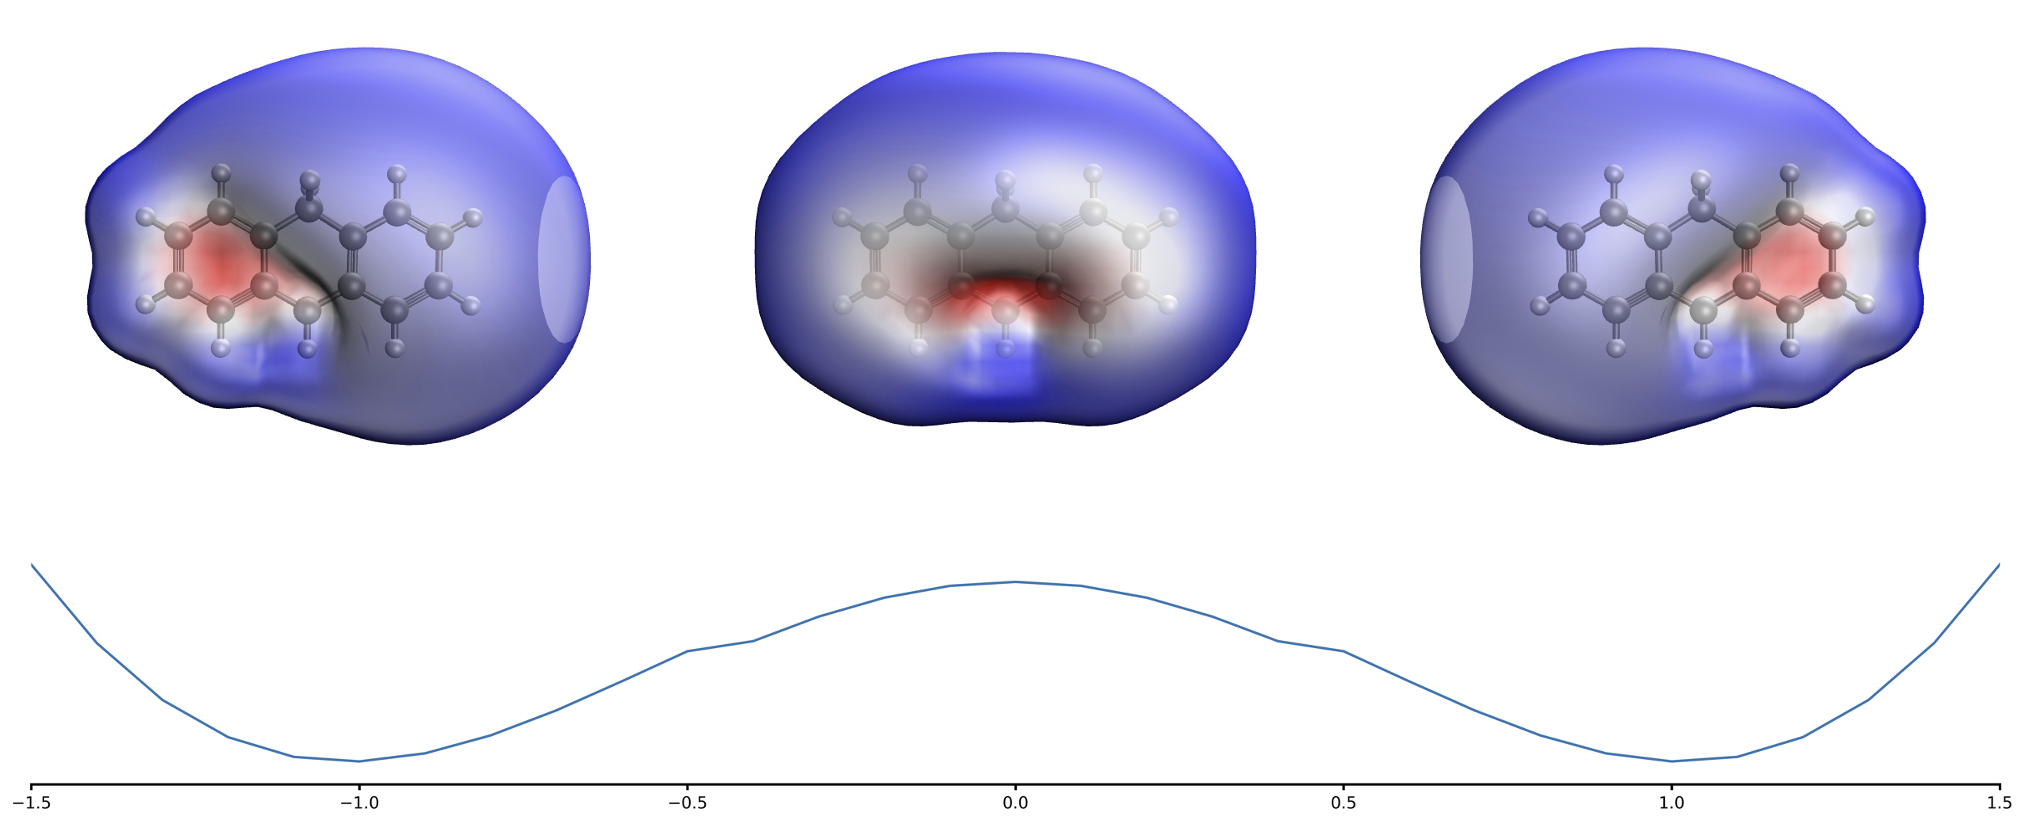
\includegraphics[width=0.8\textwidth]{figures/Fig3aa}
	\caption{dog}
	\label{Fig:3}
\end{figure}

\section{Results and Discussion}
\subsection{9H-An+}
The triple resonant photodissociation spectrum of protonated anthracene is shown in Figure~\ref{Fig:4}. The cations were prepared by resonantly ionizing the neutrals at threshold, and as such we can be certain that the spectra correspond to protonation (deuteronation) at the 9-position, the $C_{2v}$ species. The spectra reveal a number of progressions, possibly indicating a large geometry change between the ground and excited states of the cation. While the lowest energy geometry for the excited state possess $C_s$ symmetry, we may treat the excited state as approximately $C_{2v}$ as the transition state barrier (35~cm$^{-1}$) is below the zero point energy.  

\begin{figure} [h]
	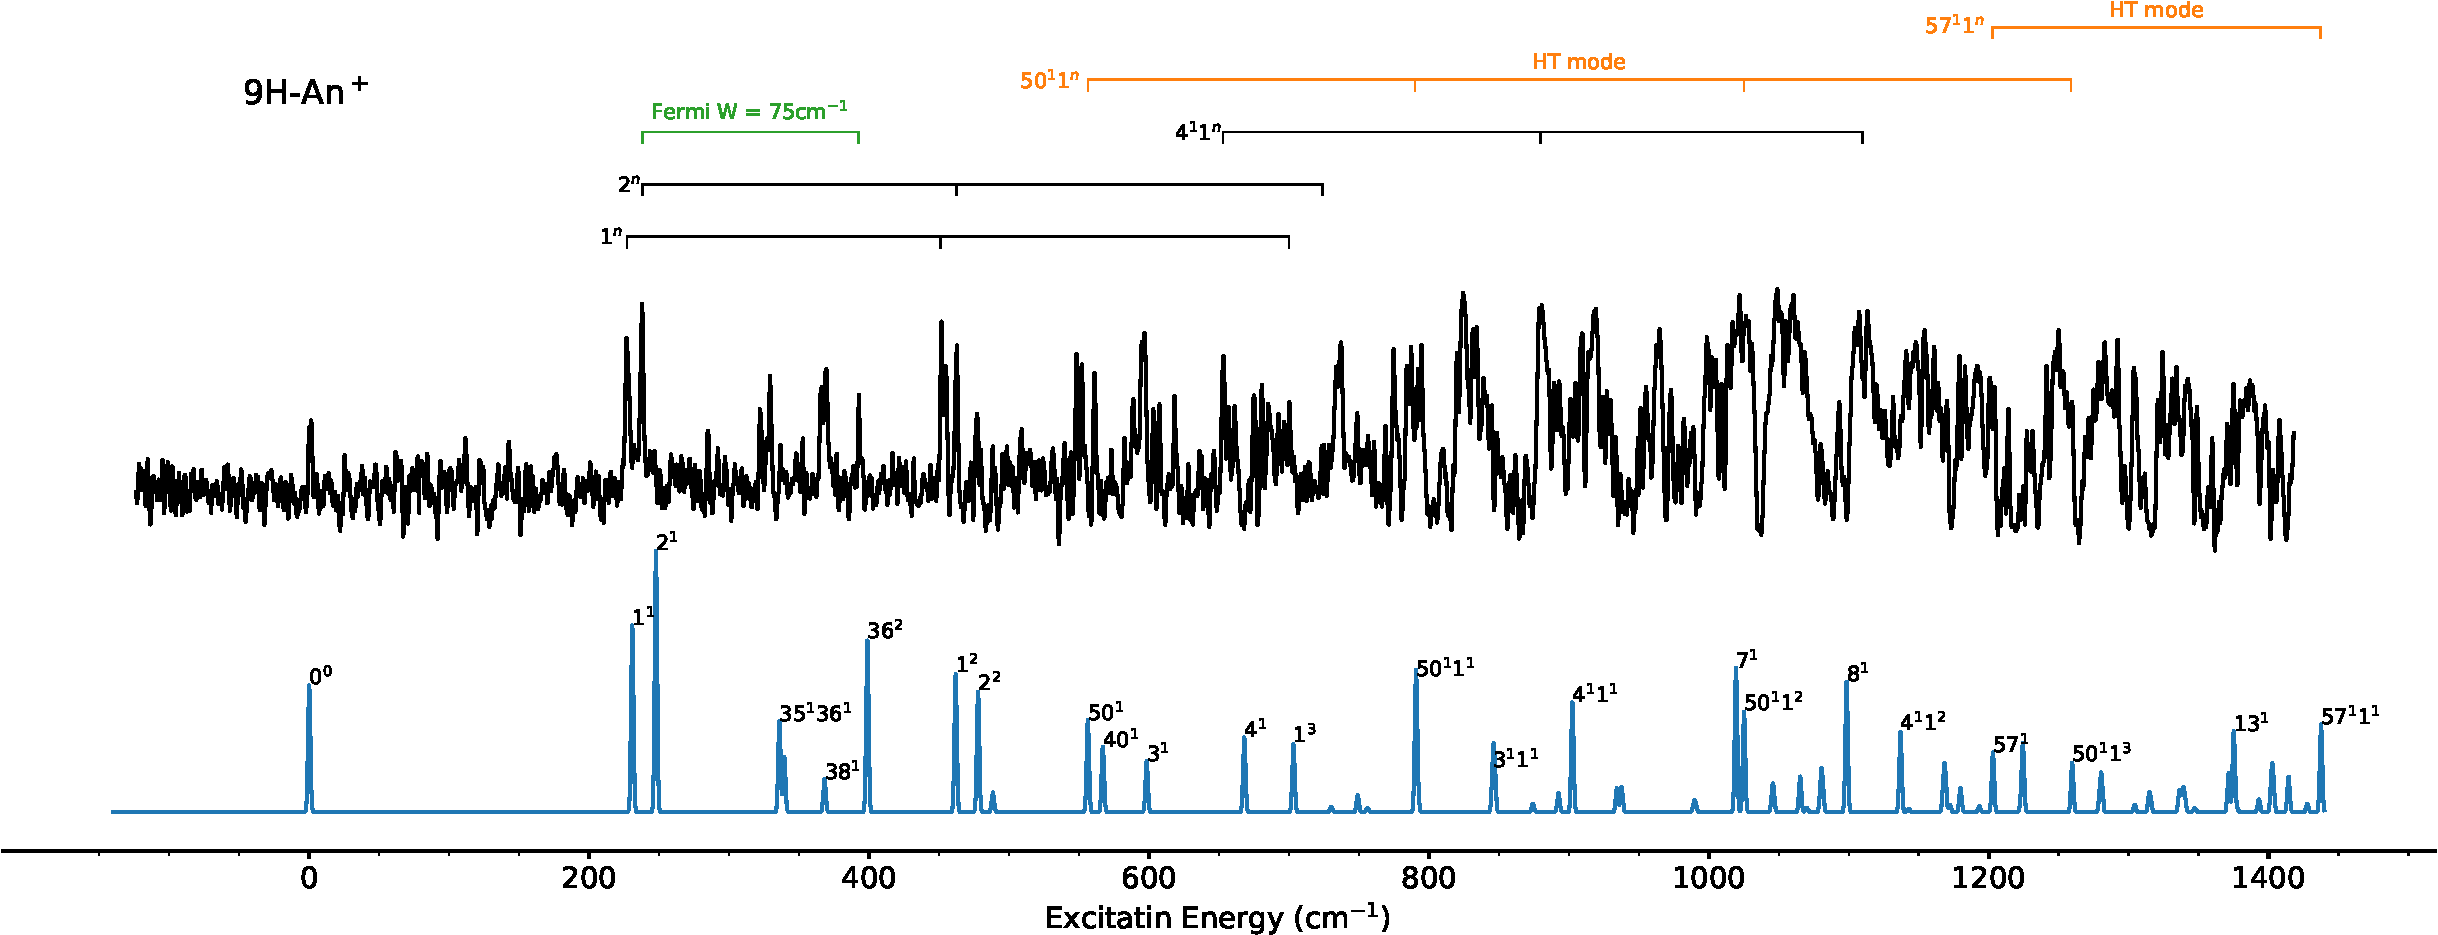
\includegraphics[width=1\textwidth]{figures/9H-An+w}
	\caption{dog}
	\label{Fig:4}
\end{figure}

The $\text{S}_0\rightarrow \text{S}_1$ origin is at 20,341~cm$^{-1}$, in agreement with the previous PIMS measurement by Alata~\emph{et al.}~\cite{ala10}, confirming their assignment to the 9H-An+ isomer. Multiple narrow transitions are observed up to 1,400~cm$^{-1}$ above the origin transition, that were not resolved in any of the previous studies. Spectral features below $\sim800~$cm$^{-1}$ appear sharp, with an average FWHM of $\sim 2.6~$cm$^{-1}$, while peaks at higher energies appear broader. This is likely due to the shorter dissociation lifetime of these excited vibrational states. It should also be noted that the relative intensity of peaks may be limited by saturation effects, where all of the resonant ground state cation signal is depleted.

As shown in Figure~\ref{Fig:4}, most of the structure observed in the experimental spectrum may be accounted for by a standard Franck-Condon (FC) simulation. Vibrational frequency calculations were computed at the M06-2X/cc-pvtz level for both the Ground $C_{2v}$ and excited transition state $C_{2v}$ geometries. Overlaps between the ground and excited state vibrational wavefunctions were then calculated, including Duschinsky rotations, to simulate the vibronic spectrum. The resulting spectrum was dominated by progressions in the $a_1$ symmetric $2^n$, $2^n$, and $4^11^n$ modes. Excellent agreement between the simulation and experiment was obtained for the $1^n$ and $4^11^n$ progressions, however the pure FC simulation did not recreate the splitting observed near $\sim230~$cm$^{-1}$. 

To evaluate whether the splitting could be caused by a 1-2 Fermi resonance with the $1^1$ transition, anharmonic frequency analysis was performed using Generalised 2nd-order Vibrational Perturbation Theory, with 3rd and 4th derivatives also calculated at the M06-2X/cc-pvtz level. This revealed a large Fermi resonance between modes v$_2$(366~cm$^{-1}$) and 2$\times$v$_{36}$(186~cm$^{-1}$), with a coupling strength
\begin{equation}
W = \frac{\sqrt{\Delta^2-\Delta_0}}{2} =75.5~\text{cm}^{-1},
\end{equation} 
where $\Delta$ is the splitting with coupling, and $\Delta_0$ is the transition separation without coupling. Hence, the doublet feature at $\sim230~$cm$^{-1}$ is not from a Fermi resonance with mode $1^1$ as was expected, but instead from a large interaction between modes $2^1$ and $36^2$. The relative intensity of of the resonant peaks is given by,
\begin{equation}
\frac{I_{v2}}{I_{2\times v36}} = \frac{\left(\Delta+\Delta_0\right)}{\left(\Delta-\Delta_0\right)}=1.08.
\end{equation}

Further features missing from the pure FC simulation may be accounted for by considering potential Herzberg-Teller vibronic coupling between the $S_1(^1A_1)$ and $S_2(^1B_2)$ excited states, as predicted from Figure~\ref{Fig:2}(b). Coupling would occur through b$_2$ vibrational promoter modes, as for $C_{2v}$ symmetry
\begin{equation}
^1A_1 \otimes b_2 = ^1B_2.
\end{equation}

To account for the nuclear-electronic interactions, the Herzberg-Teller expansion may be applied to the vibronic wavefunction of the $S_1$ state $\Psi_{S_1j}(r,Q)$. By expanding around the equilibrium geometry $Q_0$, the wavefunction may be rewritten as 
\begin{equation}
|\Psi_{S_1j} \rangle = |\psi_{S_1} \chi_{S_1j} \rangle + \gamma_{S_2k,S_1j}Q_n|\psi_{S_2} \chi_{S_2k}\rangle, 
\label{eq:shorthand}
\end{equation}
where $\psi_{S_1}$ is the electronic wavefunction of the $S_1$ state, $\chi_{S_1j}$ is the vibronic wavefunction, $Q_n$ is the coupling coordinate, and $\gamma_{S_2k,S_1j}$ is the vibronic mixing coefficient.

The strength of any vibronically coupled transitions may be determined by examining the
transition dipole moment. Substituting the $S_1$ state wavefunction from Eq.~(\ref{eq:shorthand}) into the $S_0\rightarrow S_1$ transition dipole moment gives,
\begin{align}
\mu_{\alpha}&=\langle\Psi_{S_0}|\vec{\mu}_{\alpha}|\Psi_{S_1}\rangle\\
&=\langle\psi_{S_0}|\vec{\mu}_{\alpha}|\psi_{S_1}\rangle\langle\chi_{S_0m}|\chi_{S_1j}\rangle +
\gamma_{S_2k,S_1j}\langle\psi_{S_0}|\vec{\mu}_{\alpha}|\psi_{S_2}\rangle\langle\chi_{S_0m}|Q_n|\chi_{S_2k}\rangle\\
&=\mu_{\alpha:0}^{S_1-S_0}\langle\chi_{S_0m}|\chi_{S_1j}\rangle + \gamma_{S_2k,S_1j}\mu_{\alpha:0}^{S_2-S_0}\langle\chi_{S_0m}|Q_n|\chi_{S_2k}\rangle,
\end{align}
where the term $\mu_{\alpha:0}^{S_1-S_0}= \langle\psi_{S_0}|\vec{\mu}_{\alpha}|\psi_{S_1}\rangle$ represents the $\text{S0}~\rightarrow~\text{S1}$ electronic transition moment at the ground state geometry.

Another way to describe the vibronic coupling dependence on the transition moment would be to expand the general $\mu_{\alpha:0}^{S_1-S_0}$ transition dipole function as a Taylor series in $Q_n$ about the ground state geometry,
\begin{equation}
\mu_{\alpha} = \mu_{\alpha:0}^{S_1-S_0}\langle\chi_{S_0m}|\chi_{S_1j}\rangle + \left(\frac{\partial\mu_{\alpha}^{S_1-S_0}}{\partial Q_n}\right)_0 \langle\chi_{S_0m}|Q_n|\chi_{S_2k}\rangle + \dots 
\label{eq:tm2}
\end{equation} 
Comparing Eq.~(\ref{eq:tm1}) and Eq.~(\ref{eq:tm2}) one obtains,
\begin{equation}
\left(\frac{\partial\mu_{\alpha}^{S_1-S_0}}{\partial Q_n}\right)_0 = \gamma_{S_2k,S_1j}\mu_{\alpha:0}^{S_2-S_0}.
\label{eq:tm3}
\end{equation}

This shows that the strength of the possible Herzberg-Teller transitions may be estimated, by calculating the derivative of the transition dipole moment along each $b_2$ normal mode coordinate. This was calculated for all xx modes in protonated anthracene along each axis, with the dipole derivatives given in the Supplementary information. Two vibrational modes were found to have large transition dipole moment slopes, $v_{50}$ and $V_{57}$. The transition strengths of the Herzberg-Teller coupled modes can be quantified from the TDDFT calculations by implementing a linear variation of the dipole moment to include the first order term of the Taylor expansion about the equilibrium geometry. The resulting transition intensities were added to the simulation in Figure~\ref{Fig:4}, which included two dominant progressions $50^11^n$ and $57^11^n$. 


By combining the information from the harmonic Franck-Condon, anharmonic resonances, and Herzberg-Teller calculations, the complete $S_0\rightarrow S_1$ spectrum could be simulated, as was shown in Figure~\ref{Fig:4}. The calculated spectrum resembles a close match to the experimental triple resonance spectrum, validating the shallow double well framework and $C_{2v}$ approximation used in this work to describe the system. The majority of the spectral structure can be accounted for by a series of combination bands involving the $v_1(a_1)$ symmetric in-plane wag mode, which is possibly involved in the initial excitation from the $C_{2v}$ ground state to the $C_{2v}$ excited transition state geometry. 

\subsection{Charge-Transfer Coordinate}
The molecular motion, which induces the hole-transfer from the bridging carbon to one of the aromatic rings, may be described by a combination of the normal mode coordinates. To determine which normal modes point in the same direction as the 

To inspect which vibrational modes may play a role in the hole-transfer from the bridging carbon to one of the aromatic rings,  

 transition from the initial $C_{2v}$ geometry to the $C_{s}$ geometry, 

\subsection{9D-An+}

\begin{figure} [h]
	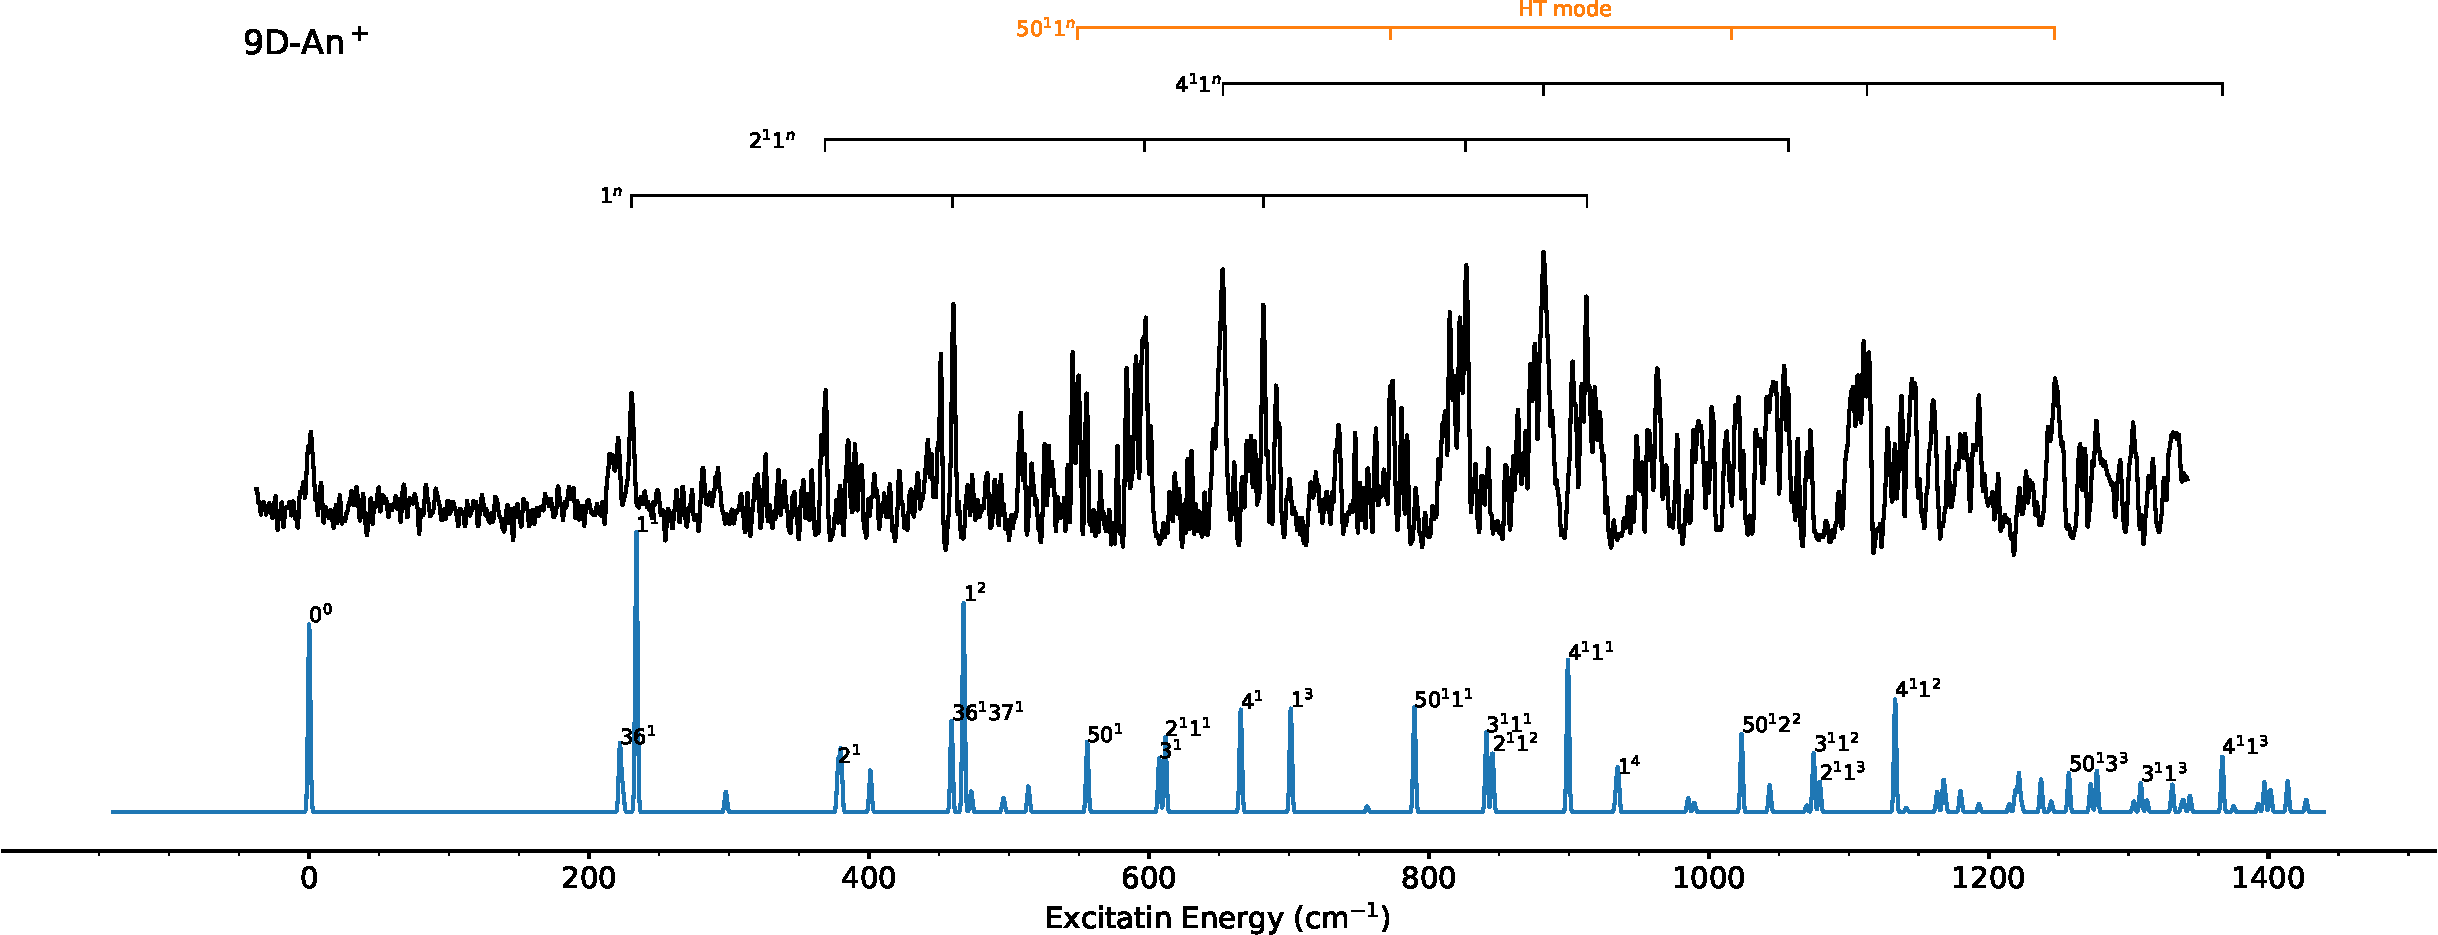
\includegraphics[width=1\textwidth]{figures/9D-An+w}
	\caption{dog}
	\label{Fig:5}
\end{figure}

\begin{acknowledgement}
	This research was supported by the Australian Research Council Discovery
	Project Grant DP190103151.  
\end{acknowledgement}

% Create the reference section using BibTeX: 
\bibliography{AnH+}

\newpage
\onecolumn
\subsection{TOC Graphic - For Table of Contents Only}
\vspace{2ex}
\begin{center}
%	\includegraphics[width=8.5cm]{figures/TOC}
\end{center}

\end{document}
% ****** End of file apstemplate.tex ******